\label{ch:background}

This work combines results from the field of reinforcement learning and wind turbine control. This chapter gives an introduction to extracts from both fields, focussing on concepts that are relevant to the approach.

\section{Reinforcement Learning}
\label{section:background-reinforcement-learning}
\begin{summary}
In this section, we will introduce fundamental concepts of reinforcement learning with a specific focus on the \ac{SAC} algorithm by \citet{haarnojaSoftActorCriticOffPolicy2018}, as this algorithm is primarily used in this work. Most of the theory is generally applicable and not limited to this algorithm.
\end{summary}

\subsection{Fundamentals}

\begin{summary}
This subsection defines the mathematical notion of environments and rewards, through which reinforcement learning interfaces with the problem at hand. At every time step, a state and a reward from the environment are the input to the reinforcement learning algorithm, which in turn produces an action for this time step to maximize reward. 
\end{summary}

The fundamental concept of reinforcement learning is shown in Figure \ref{fig:rlcycle}. The \textit{agent} produces \textit{actions} in a given \textit{environment}. The environment in turn gives a \textit{state} and a \textit{reward}, judging the quality of the state. Eventually, a \textit{policy} which produces optimal actions for all states with respect to the reward is to be learnt.

\begin{figure}
\centering
  \begin{tikzpicture}[node distance=3cm]
    \node (agent) [process] {Agent};
    \node (environment) [process, below of=agent] {Environment};

    \draw [arrow,out=210,in=150] (agent.west) to node[left]{action $a$} (environment.west);
    \draw [arrow,out=30,in=330] (environment.east) to node[right,text width=2cm]{state $s$,\\reward $r$} (agent.east);
  \end{tikzpicture}

  \caption{The reinforcement learning interaction cycle}
  \label{fig:rlcycle}
\end{figure}

An environment is either a simulation or a real world environment, which enables interaction in a time-discrete manner. Each time step, the environment produces a state $s \in S$ and a reward signal $r(s,a): S \times A \rightarrow [\rmin, \rmax]$ upon receiving an action $a \in A$. If $A \in \mathbb{R}^n$ the problem is called \textit{continuous control} reinforcement learning, opposed to \textit{discrete control} with $A$ being a finite set of possible actions. It is usually required for the environment to be a \textit{Markov Decision Process}, meaning the probability of landing in a state $s_t$ at time step $t$ is only dependent on the previous time step state $s_{t-1}$ and action $a_{t-1}$, not of any other time steps. Formally, this writes: $Pr(s_t | a_{t-1}, s_{t-1}, a_{t-2}, ... , s_0) = Pr(s_t | a_{t-1}, s_{t-1})$, with $Pr(x|y)$ denoting the conditional probability of $x$ under condition $y$. When the state does not contain all information necessary to determine a state transition in the environment, the decision process is called \acf{POMDP}. In \ac{RL}, \acp{POMDP} are commonly assumed. The unknown environment dynamics are denoted by $\rho(s_{t+1}|s_t,a_t): S \times S \times A \rightarrow [0, \infty)$, giving the probability density for reaching a state $s_{t+1}$ from a state $s_t$ and an action $a_t$. Furthermore, we denote the unknown initial state distribution by $\rho_0(s_0) : S \rightarrow [0,1]$. A trajectory, also called rollout, is a list of succeeding states and actions: $\trajectory = (s_0, a_0, s_1, a_1, ..., s_t, a_t)$. A trajectory can be sampled from an environment until a stop condition is reached, which can be a signal implemented in the environment or a constant maximum horizon $\lambdatraj$ such that $t < \lambdatraj \forall t$.

The agent has the aim of finding an optimal policy for the environment which produces the maximum cumulative reward. A policy gives an action for each state. There are stochastic policies $\pi : S \times A \rightarrow [0,1]$, giving a probability distribution over actions for a state, and deterministic policies $\pi_{\text{det}} : S \rightarrow A$. As stochastic policies output a probability for an action, the notation $\pi(a|s)$ is used in accordance to conditional probability notation. If the action is not of interest, we write $\pi(\cdot|s)$. A stochastic probability can be evaluated deterministically with $\pi_{\text{det}}(s) = \argmax_{a} \pi(a|s)$. If a policy is from a class of functions parametrized by $\theta$, we write $\pi_{\theta}$. We denote $\rho_{\pi}(s, a)$ as the state-action marginals induced by the policy $\pi$ in the unknown environment dynamics $\rho$ and similarly $\rho_{\pi}(s)$ as the state marginals. Formally, state-action marginals can be expressed by summing trajectory marginals over all possible trajectories as in Equation \ref{eq:state-action-marginals}:

\begin{equation}
  \rho_{\pi}(s, a) = \sum_{\trajectory} \left[ \left. \rho_0(s_0) \prod_{t=0} \pi(a_t | s_t) \rho(s_{t+1}|s_t, a_t) \right| s_0, s_t, a_t \in \trajectory \right]
  \label{eq:state-action-marginals}
\end{equation}

The aim of reinforcement learning is to find a policy which maximizes the expected reward over time, or maximizing Equation \ref{eq:policy_objective_basic}:

\begin{equation}
\label{eq:policy_objective_basic}
\mathcal{J}_{\pi} = \sum_t \mathbb{E}_{(s_t, a_t) \backsim \rho_{\pi}} [\gamma^t r(s_t, a_t)]
\end{equation}

The discounting factor $\gamma \in [0,1]$ is used to prevent summing to infinity for settings in which $t$ is positively unbounded (also called \textit{infinite-horizon} settings). Usually, a value close to $1$ is used for $\gamma$ such as $0.99$. $\mathcal{J}_{\pi}$ denotes the optimization aim for the policy, which is to be maximized.


\subsection{Q-Learning With The Bellman Backup}
\label{section:background-q-learning}

\begin{summary}
This subsection gives an insight into Q-Learning, which is a technique to estimate the expected return for all states and actions. Knowing the Q-Function for an environment allows to choose the optimal action for a given state by finding the action argument which maximizes the Q-Function. Several techniques are introduced that allow for an efficient and unbiased Q estimation with neural networks.
\end{summary}

It is desirable to know how much accumulated reward (\textit{return}) is to be expected when taking an action in a specific state. Assuming perfect knowledge of expected returns, a perfect policy could be constructed by always choosing the action for any state that gives the highest expected return. A \textit{Q-function} $Q : S \times A \rightarrow \mathbb{R}$ is commonly used in reinforcement learning to estimate expected discounted return for a state and an action. This Q-function can then either be used directly for choosing the optimal action for a state like in \citet{mnihHumanlevelControlDeep2015}, or to derive a policy gradient. Finding the optimal action is non-trivial in continuous action spaces, especially with non-linear Q-function approximators like neural networks, for which the argmax is not trivially found. Hence, a policy is generally used in continuous action spaces. Fitting this Q-function happens through the recursive Bellman Backup Operator \cite{richardbellmanTheoryDynamicProgramming1954} as presented in Equation \ref{eq:bellman-backup} or a variation of it:

\begin{equation}
Q(s_t, a_t) = r(s_t, a_t) + \gamma Q(s_{t+1}, a_{t+1})
\label{eq:bellman-backup}
\end{equation}

If actions are chosen by the optimal policy, we write $Q^*$, and if actions are chosen by any other policy $\pi$, we write $Q^{\pi}$. This construct is proven to converge towards the ground-truth value \cite{meloConvergenceQlearningSimple2001}. Also, it is possible to optimize a parametrized Q-function $Q_{\theta}$ using gradient ascend (or gradient descend on the inverse) on the optimization aim $\mathcal{J}_{Q}$ for the Q-function from Equation \ref{eq:q-optimization-aim}:

\begin{equation}
\mathcal{J}_{Q_{\theta}} = -\frac{1}{2} (Q_{\theta}(s_t, a_t) - \hat Q(s_t, a_t))^2
\label{eq:q-optimization-aim}
\end{equation}

with $\hat Q(s_t, a_t) = r(s_t, a_t) + \gamma Q_{\theta}(s_{t+1}, a_{t+1})$ and gradients not propagating through $\hat Q$. When $a_{t+1}$ is sampled from a policy during the update, this specific way to optimize the Bellman equation is also called \textit{Temporal Difference learning (TD-learning)}. When $a_{t+1}$ only comes from experience, it is called \textit{SARSA}. 

In practice, instabilities arise, especially when the Q-function approximator is a large and non-linear function approximator such as a neural network. One fix for these instabilities is to use a \textit{target network} for the target Q values of Equation \ref{eq:q-optimization-aim} as $\hat Q(s_t, a_t) = r(s_t, a_t) + \gamma Q_{\bar{\theta}}(s_{t+1}, a_{t+1})$. Note the different parametrization by $\bar{\theta}$. These target networks are a copy of the main network and receive parameter updates from the main network in a delayed manner. In \citeapos{mnihHumanlevelControlDeep2015} \ac{DQN} algorithm, parameters are copied from main to target network every $n$ algorithm iterations, while in \citeapos{lillicrapContinuousControlDeep2019} \ac{DDPG} algorithm  parameters are continually being copied over using a smooth target update: $\bar{\theta}' = \targetupdate \bar{\theta} + (1-\targetupdate)\theta$ with $\theta$ being the parameters of the main network and $\bar{\theta}$ the parameters of the target network. The target update coefficient $\targetupdate \in [0,1]$ dictates how fast the target is receiving parameter updates from the main network, with lower values of $\targetupdate$ meaning closer ties between main and target. Typically, a relatively high value such as $\targetupdate = 0.95$ is used.

Further experience has shown that approximation errors overestimating the ground-truth value of $Q$ propagate through the Bellman Backup easier than underestimations, resulting in a phenomenon called overestimation bias. \citet{hasseltDoubleQlearning2010} have investigated this problem and proposed to fit two Q-functions, which is used in \citeapos{fujimotoAddressingFunctionApproximation2018} \ac{TD3} algorithm. Inference is done by taking the minimum of the two Q-functions, reducing overestimation bias and improving algorithmic performance. 

In some algorithms, a value function $V : S \rightarrow \mathbb{R}$ is used instead of a Q-function, where the value function can be defined with help of the Q-function: $V(s_t) = \mathbb{E}_{a_t \backsim \pi} Q(s_t, a_t)$.

\subsection{Policy-based Methods}

\begin{summary}
This subsection introduces policy based methods of reinforcement learning, which utilize a second neural network that returns an action for a given state. This neural network is trained with the help of the Q-function. Using a policy improves training stability especially in continuous action spaces.
\end{summary}

In discrete action spaces, a greedy policy can be derived from the Q-function directly by using $\pi(s) = \argmax_a Q(s,a)$. In continuous action spaces, the Q-function can not be used to derive a policy directly as finding the $\argmax_a$ over a continuous action space and a non-linear Q-function approximator is non-tractable. However, having a Q-function, we can substitute our policy optimization aim from Equation \ref{eq:policy_objective_basic} yielding Equation \ref{eq:policy-objective-q}:

\begin{equation}
  \mathcal{J}_{\pi} = \sum_t \mathbb{E}_{(s_t \backsim \rho, a_t \backsim \pi(s_t))} [\gamma^t Q(s_t, a_t)]
  \label{eq:policy-objective-q}
\end{equation}

This objective can directly be optimized, as the Q-function approximation through a neural network is differentiable. Integrating Q-functions into the policy update, instead of computing the gradient estimations over recently sampled transitions, yields a range of advantages with the most notable being better sample efficiency. It is not necessary to gather a high number of samples for each policy update, as the Q-function implicitly stores information about the reward function. The resulting construct is called \textit{actor-critic}, with the actor being the policy and the critic the Q-function. 

When the experiences $(s_t, a_t)$ are sampled freshly with the updated policy and old experiences are discarted, this is called \textit{on-policy} learning. The alternative to this is \textit{off-policy} learning, where the most recent samples are stored in a \textit{replay buffer} $\replaybuffer$ and sampled from there. Furthermore, there exists a differentiation between \textit{online} RL, which can sample from an environment and \textit{offline} RL, which is only presented with a replay buffer. 

Concurrently updating the Q-function approximator and the policy comes with the disadvantage that the samples the Q-function learned from were generated by an older policy. The current policy might perform differently, giving a wrong Q estimate and hence a wrong gradient direction on the policy gradient. This problem is especially pronounced when using older samples from a replay buffer, but it is nevertheless possible to formulate a policy gradient as shown by \citet{degrisOffPolicyActorCritic2013}. In practice, on-policy algorithms tend to be more stable while requiring more samples to train.

\subsection{Intuition}

\begin{summary}
This subsection tries to convey an intuition on how Q-learning and policy optimization together can form a working actor-critic reinforcement learning algorithm.
\end{summary}

The Q-function is fit to represent expected return, which is the exact quantity subject to optimization. More specifically, the aim is to know the action in each state that brings the highest expected return. Repeated application of the recursive Bellman backup (Equation \ref{eq:bellman-backup}) is proven to yield a Q approximation, which converges to the optimal Q-function $Q^*$. Fitting this approximator instead of optimizing returns directly through intensive sampling makes the process much more tractable. Especially because the environment in \textit{model-free} RL does not offer the option to reset to a certain state. Without the Q approximation, an exhaustive tree search would be required to know the best action for each state. Such a tree search is a common procedure in \textit{model-based} RL, where the agent has the option to set the environment to a certain state. AlphaGo \cite{silverMasteringGameGo2016}, the algorithm that beat the Go champion Lee Sedol, uses a Monte-Carlo Tree Search augmented with a value function.

Knowing the optimal Q-function $Q^*$, the best possible action for a specific state can be found by computing Q values for all allowed actions in that state and choosing the argmax. In a discrete action space setting, this is a common procedure \cite{mnihPlayingAtariDeep2013}, whereas in a continuous action space, it would be required to resort to some form of optimization algorithm to find the best action from the infinite set of possibilities. To avoid this, a common practice is to fit a policy, which allows obtaining the best action in a single forward pass. It is possible to compute a black-box gradient across the unknown environment dynamics, which constitutes the original policy gradient algorithm \cite{suttonPolicyGradientMethods2000}. However, using a neural network for the Q-function approximation offers the possibility of directly backpropagating gradients through the Q-function. The gradients at the output side of the Q-function point in the direction of better returns, hence the gradients at the action input point in the direction of better actions. Further backpropagating these action gradients from the Q-function into the policy parameters yields gradients pointing in the direction of better policy parameters, which can be used the traditional way for stochastic gradient descend or other first-order optimizers.


\subsection{Smoothness Regularization}
\label{section:background-smoothness-regularization}

\begin{summary}
This subsection introduces smoothness regularization techniques, which are beneficial in the wind turbine environment. Wind turbines react sensibly to noise and a noisy control policy is detrimental to performance. Disabling policy noise altogether is not possible, as it would destabilize Q-function estimation. Hence, we present a separate regularization technique to incentivize smooth control.
\end{summary}

Continuous control reinforcement learning policies are not directly incentivized to yield smooth policies. However, for some problems, a smooth policy can improve final performance or other secondary metrics. During our work, we have observed learnt policies to produce highly noisy actions over time. To our knowledge, two works have analyzed this problem in detail. \citet{shenDeepReinforcementLearning2020} investigate spatial regularization both in the policy and Q-function updates and evaluate different forms of spatial regularizations. Their results have shown no significant difference between applying the regularization in the policy or Q update. \citet{mysoreRegularizingActionPolicies2021} only apply regularizations to the policy update but propose both spatial and temporal regularization. Their results have shown their additional temporal regularization to be highly beneficial. Hence, we will focus on \citeapos{mysoreRegularizingActionPolicies2021} solution \acf{CAPS} for this work.

\textit{Spatial smoothness regularization} works by penalizing a high difference in policy output (action) for a small difference in policy input (state):

\begin{equation}
  \capss = \lambdaspat D(\pi(s), \pi(\tilde s))
\end{equation}

with a distance measure $D$, a state $s$ and a second state $\tilde s$ which is obtained by adding a small perturbation to $s$. \citet{mysoreRegularizingActionPolicies2021} propose a perturbation in the form of spherical Gaussian noise: $\tilde s = s + \mathcal{N}(0, \epsilon_{s})$ and the euclidean distance as distance measure $D$.

\textit{Temporal smoothness regularization} works by penalizing a high difference in policy output for two subsequent states as policy input:

\begin{equation}
  \capst = \lambdatemp D(\pi(s_t), \pi(s_{t+1}))
\end{equation}

with a distance measure $D$ and states from two subsequent time steps $s_t$ and $s_{t+1}$. \citet{mysoreRegularizingActionPolicies2021} propose the euclidean distance as distance measure $D$.

Both regularization penalties are subtracted from the policy optimization aim:

\begin{equation}
  \mathcal{\tilde J}_{\pi} = \mathcal{J}_{\pi} - \capss - \capst
  \label{eq:smoothness-regularized-policy}
\end{equation}

This works regardless of the actual policy optimization aim $\mathcal{J}_{\pi}$ and thus is applicable to a wide range of continuous control reinforcement learning algorithms. The results of both regularizations are significantly smoother policies and better sample efficiency and training stability.

% \subsection{Value regularization}
% \label{section:background-value-regularization}
% \todo{Decide whether to drop this section or to leave it in, as it's quite a theoretical stretch to bring this to work. When leaving in, connect it to the work.}
% \citet{kumarDR3ValueBasedDeep2021} discover an implicit regularization in value-based TD-learning, which incentivizes high \textit{feature co-adaptation} and thus leads to unlearning and poor stability in offline RL. They define feature co-adaptation as the dot-product of the last-layer activations of the Q-function for the current and next timestep states and actions: $\qlastlayer(s_t, a_t)^\intercal \qlastlayer(s_{t+1}, a_{t+1})$ where $\qlastlayer(s,a)$ is the activation of the last layer of the Q-function before the layer that reduces the latent features to the actual Q-value. A high feature co-adaptation means either a high cosine similarity of the two last-layer activations or high norms, as the dot-product can be written as $\text{dot}(a,b)=|a| |b| \cos(a \measuredangle b)$. Hence, the degree of feature co-adaptation is a measure of similarity. While a certain degree of similarity from the last feature representation to the next might be inherent to the ground truth Q-function, too much similarity reduces the ability to derive a sensible policy gradient along the Q-function.

% In \cite[Equation 7]{kumarDR3ValueBasedDeep2021}, they propose an explicit regularization as shown in Equation \ref{eq:dr3-regularization} that counteracts the implicit maximization of feature co-adaptation:

% \begin{equation}
%   \drrrreg = \drrrcoeff \frac{1}{|D|} \sum_{s_t, a_t, s_{t+1}, a_{t+1} \backsim D} \qlastlayer(s_t, a_t)^\intercal \qlastlayer(s_{t+1}, a_{t+1})
%   \label{eq:dr3-regularization}
% \end{equation}

% with the current and next state actions being sampled from the replay buffer $D$ in batches of size $|D|$. $\drrrcoeff$ is a coefficient that controls the magnitude of regularization and needs to be tuned to each environment. \todo{include into sac section}

% Albeit the theory applies to general TD-learning, the work of \citet{kumarDR3ValueBasedDeep2021} only analyzes the offline RL task. In offline RL, a policy should be learnt only from expert demonstrations without the possibility to sample from an environment. During the poster session at the NIPS 2021 conference, they orally mentioned brief experiments with online off-policy RL, which did not show the problem, and henceforth did not include any references to online RL in their publication. We use it nevertheless, as we hypothesize feature co-adaptation to pose a problem in wind turbine reinforcement learning.

\subsection{Smoothness-regularized Soft Actor Critic}
\label{section:background-sac}

\begin{summary}
This subsection discusses the algorithm that is used in most parts of this work. The results of all previous background sections is put together to form an algorithm. We implement the \acf{SAC} algorithm by \citet{haarnojaSoftActorCriticOffPolicy2018} with improvements from \citet{haarnojaSoftActorCriticAlgorithms2019}. Furthermore, a smoothness regularization after \citet{mysoreRegularizingActionPolicies2021} has been applied. 
\end{summary}

\citet[Equation 1]{haarnojaSoftActorCriticOffPolicy2018} use a modified optimization goal to the vanilla optimization goal presented in \ref{eq:policy_objective_basic}. This \textit{entropy augmented} optimization goal is as shown in Equation \ref{eq:soft-policy-objective}:

\begin{equation}
\label{eq:soft-policy-objective}
\mathcal{J}_{\pi} = \sum_{t=0}^{\infty} \mathbb{E}_{(s_t, a_t) \backsim \rho_{\pi}} [r(s_t, a_t) + \alpha \mathcal{H}(\pi(\cdot|s_t))
\end{equation}

with $\alpha$ being an entropy temperature coefficient and $\mathcal{H}(\pi(\cdot|s_t))$ denoting the entropy of the policy for state $s_t$. Entropy can be computed as $\mathcal{H}(\pi(\cdot|s)) = - \int \pi(a | s) \log \pi(a | s) da$ for any probability distribution. In practice, multivariate Gaussians, usually even with a diagonal covariance matrix, are commonly used to represent the policy distributions, hence the entropy can be obtained directly as a function of the covariance matrix without involving integration. If no closed-form expression of the entropy exists, \citet{haarnojaReinforcementLearningDeep2017} have proposed an adaptation. The entropy augmented optimization goal forms a branch called \textit{Maximum Entropy} Reinforcement Learning, as we are maximizing both reward and policy entropy. Through the temperature coefficient $\alpha$, the exploration-exploitation trade-off can be explicitly controlled, with a higher $\alpha$ resulting in more exploration. A discounting factor $\gamma$ can be used with the entropy augmented optimization goal to incorporate infinite-horizon settings; we refer to their proof in Appendix A of their publication \cite[Appendix A]{haarnojaSoftActorCriticOffPolicy2018}. Through maximizing Equation \ref{eq:soft-policy-update}, a policy approximator $\pi_{\vartheta}$ parametrized by $\vartheta$ can be optimized:

\begin{equation}
  \mathcal{J}_{\pi}(\vartheta) = \mathbb{E}_{(s_t \backsim \replaybuffer, a_t \backsim \pi_{\vartheta})} \left[Q_{\theta}(s_t, a_t) - \alpha \log(\pi_{\vartheta}(a_t | s_t))  \right]
  \label{eq:soft-policy-update}
\end{equation}

Note the subtraction of the policy entropy, which is motivated in \cite[Equation 4]{haarnojaSoftActorCriticAlgorithms2019}. Through the reparametrization trick \cite[Equation 8,9]{haarnojaSoftActorCriticAlgorithms2019}, gradients can be back-propagated directly through the stochastic policy when sampling $a_t \backsim \pi_{\vartheta}$. Integrating the smoothness reqularization by \citet{mysoreRegularizingActionPolicies2021} is possible as in Equation \ref{eq:smoothness-regularized-policy}. \citet[Chapter 5]{haarnojaSoftActorCriticAlgorithms2019} also present a heuristic to automatically tune the entropy temperature coefficient $\alpha$ as in Equation \ref{eq:sac-entropy-heuristic}:

\begin{equation}
  \mathcal{J}(\alpha) = \mathbb{E}_{a_t \backsim \pi} \left[\alpha \log \pi(a_t | s_t) + \alpha \targetentropy \right]
  \label{eq:sac-entropy-heuristic}
\end{equation}

with $\targetentropy$ denoting the target entropy hyperparameter. To work with the entropy augmented policy objective, an entropy augmented Bellman backup as described in Equations \ref{eq:soft-q-update}, \ref{eq:soft-q-update-value} is used:

\begin{equation}
  \mathcal{J}_Q(\theta) = \mathbb{E}_{(s_t, a_t, s_{t+1}) \backsim \replaybuffer} \left\{ -\frac{1}{2} \left[ Q_{\theta}(s_t, a_t) - (r(s_t, a_t) + \gamma V(s_{t+1}) )\right]^2 \right\}
  \label{eq:soft-q-update}
\end{equation}

\begin{equation}
  V(s_{t+1}) = \mathbb{E}_{a_{t+1} \backsim \pi} \left[ Q_{\bar{\theta}} (s_{t+1}, a_{t+1}) - \alpha \log(\pi_{\vartheta}(a_{t+1} | s_{t+1}) \right]
  \label{eq:soft-q-update-value}
\end{equation}

with $\replaybuffer$ being a replay buffer of recently sampled transitions. Furthermore, they employ common techniques for improving Q function convergence through target networks with smooth parameter updates and two Q-functions, making for a total of four Q-function approximators.

The resulting algorithm is a smoothness-regularized online off-policy actor-critic maximum- entropy reinforcement learning algorithm. It offers the advantage of good sample efficiency that comes with off-policy algorithms, an option to control the exploration-exploitation trade-off and good empirical performance. It does not exhibit high hyperparameter sensitivity such as \ac{TD3} and reaches stability levels close to \ac{PPO}, and as such has become a de-facto standard in RL.

\section{Wind Turbine Control}
\label{section:background-wind-turbine-control}

\begin{summary}
In this Section, we will describe the fundamentals of wind turbine control with a specific focus on the IEA-10MW offshore turbine \cite{bortolottiIEAWindTCP2019}, as most of this work deals with this specific turbine. However, the theory applies to any \ac{HAWT}.
\end{summary}

\subsection{Wind Turbine Fundamentals}
\label{section:background-wind-turbine-fundamentals}

\begin{summary}
This subsection introduces components of a wind turbine and the rated speed concept. The rated wind speed is a wind speed at which the wind turbine generator is saturated. Below rated wind, a power maximizing control strategy is used, and above rated wind, a load minimizing control strategy. The above-rated regime is the main focus of this work, as we try to learn a load minimizing control strategy.
\end{summary}

\begin{figure}
  \centering
  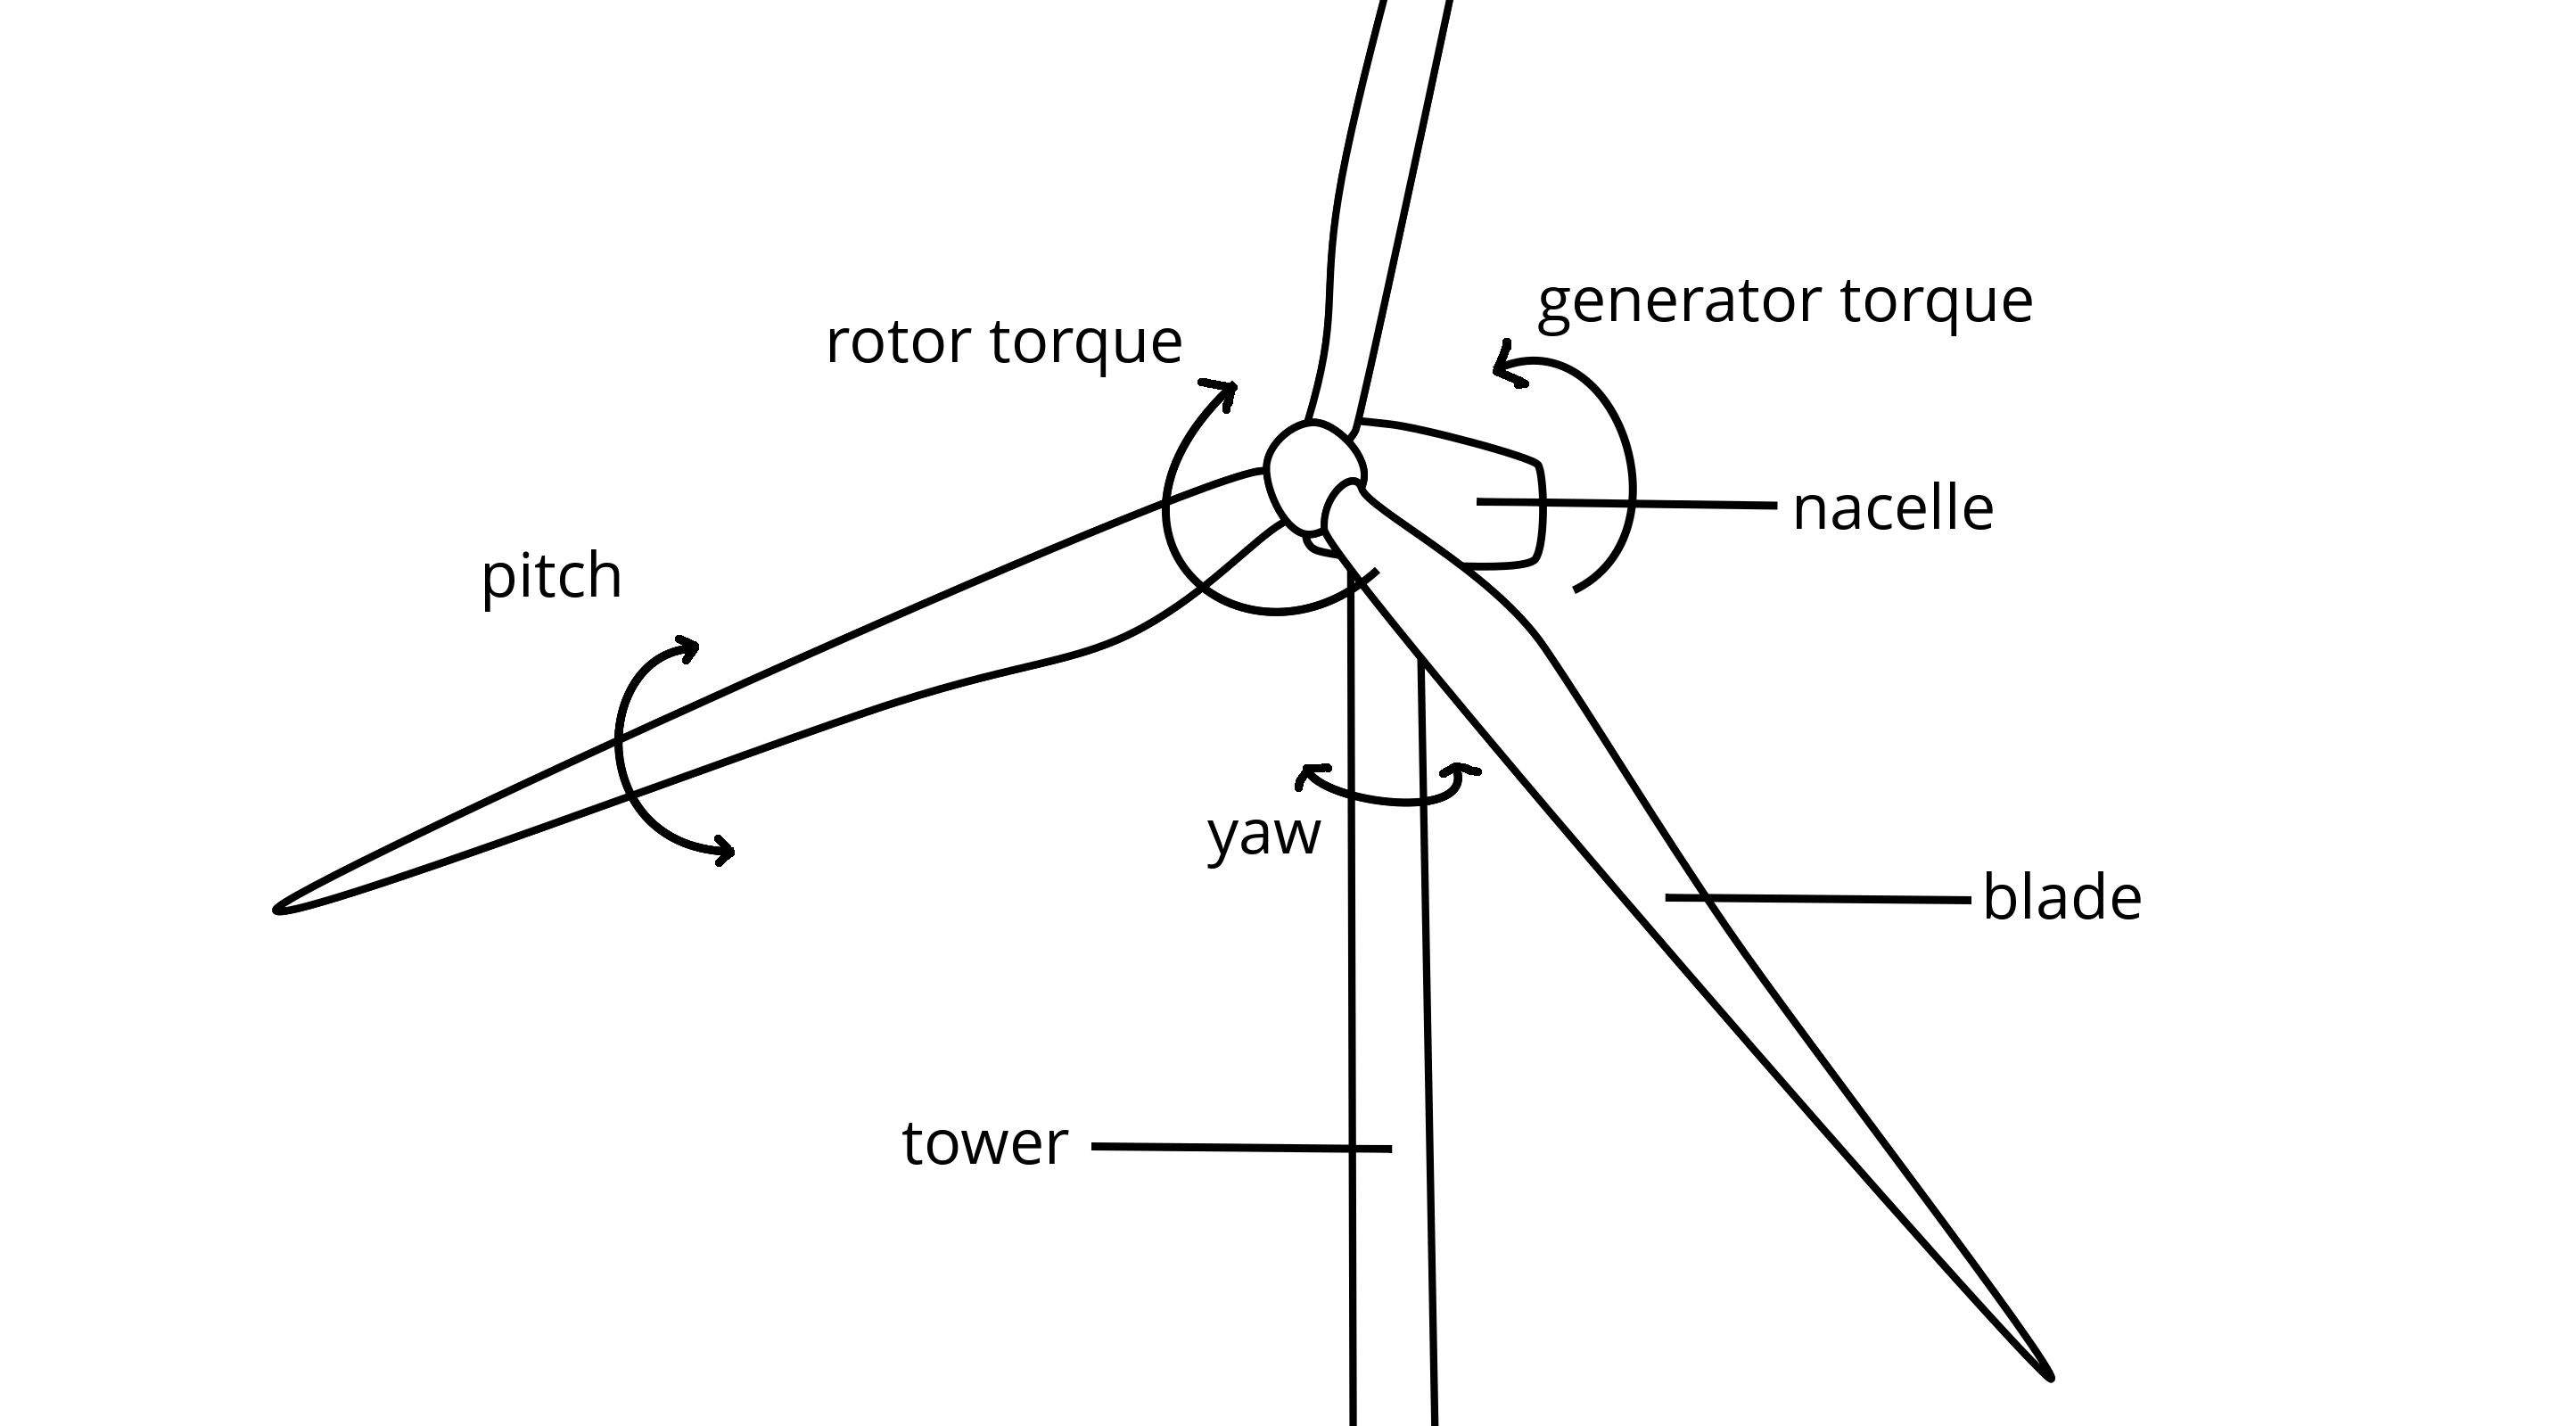
\includegraphics[width=0.7\textwidth]{images/Windturbine-Schema.png}
  \caption{A schema of the most important wind turbine components and control actions. Based on \cite{openclipartWindTurbineSketch2017}}
  \label{fig:windturbine-schema}
\end{figure}

% There are two major types of wind turbines, \acfp{VAWT} and \acfp{HAWT}. The latter proved to be suited better for large scale applications , hence we will focus this work purely on that type.
A \acf{HAWT} is the most prominent turbine design for large scale applications\cite[Chapter 1.1]{burtonWindEnergyHandbook2011}. It consists of the components shown in figure \ref{fig:windturbine-schema}. A \textit{nacelle} sits on top of a \textit{tower}. The nacelle holds a horizontal shaft with usually three \textit{blades} attached. The blades create \textit{rotor torque} through aerodynamic lift, the force that spins the rotor. The shaft is connected to a \textit{generator} inside the nacelle, which converts the rotational energy of the shaft to electric energy by applying a counteracting \textit{generator torque}. If generator torque and rotor torque match, the rotor speed stays level. The act of turning the entire nacelle on top of the tower to face the wind is called \textit{yaw} and is typically done by a yaw motor. Furthermore, the blades can be rotated along their root to tip axis to change their aerodynamic response to the incoming wind, which is called \textit{pitch}.

\begin{figure}
  \centering
  \begin{subfigure}[b]{0.32\textwidth}
      \centering
      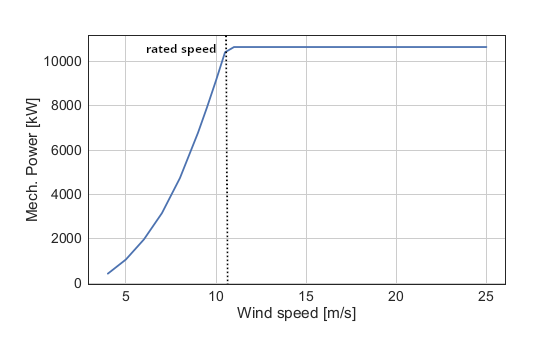
\includegraphics[width=\textwidth]{images/IEA10MW-Characteristics-1.png}
      \caption{Power production}
      \label{fig:IEA10MW-power}
  \end{subfigure}
  \begin{subfigure}[b]{0.32\textwidth}
      \centering
      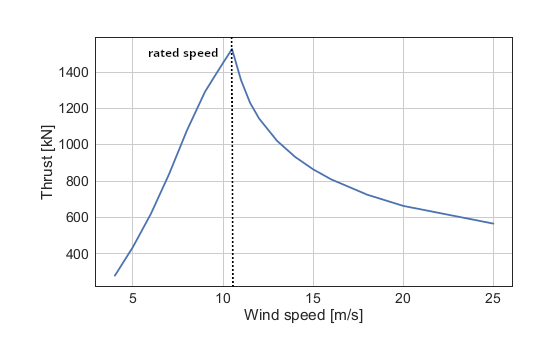
\includegraphics[width=\textwidth]{images/IEA10MW-Characteristics-2.png}
      \caption{Rotor thrust}
      \label{fig:IEA10MW-thrust}
  \end{subfigure}
  \begin{subfigure}[b]{0.32\textwidth}
    \centering
    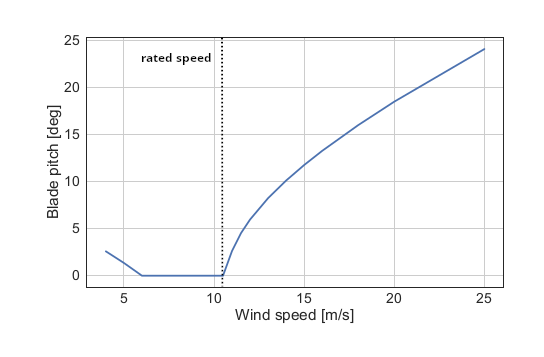
\includegraphics[width=\textwidth]{images/IEA10MW-Characteristics-3.png}
    \caption{Base pitch}
    \label{fig:IEA10MW-pitch}
  \end{subfigure}
  \caption{The steady wind operation of the 10MW IEA turbine from \citet[Figure 33]{bortolottiIEAWindTCP2019}}
  \label{fig:IEA10MW}
\end{figure}

Typically, \acp{HAWT} are designed with a specific \textit{rated wind speed} \cite[Chapter 6.3]{burtonWindEnergyHandbook2011}. This wind speed is the point above which the rotor yields more energy than the generator can convert. To prevent overheating of the generator, the aerodynamic torque produced by the rotor needs to be limited. This happens by increasing the pitch of the blades, reducing their aerodynamic efficiency. The IEA-10MW turbine has a rated wind speed of $10.75 \frac{\text{m}}{\text{s}}$ \cite[Table 16]{bortolottiIEAWindTCP2019}. In figure \ref{fig:IEA10MW} this point is visible in all three plots. Subfigure \ref{fig:IEA10MW-power} displays mechanical rotor power over wind speed, which is equal to electric turbine output, ignoring minor energy losses in the drive train, generator and inverter. From rated wind speed up, power plateaus at the rated power output, while below rated it gradually increases to maximum level. To prevent further power increase, the blade pitch angle in Subfigure \ref{fig:IEA10MW-pitch} is increased gradually from rated wind speed up, reducing aerodynamic rotor efficiency. The reduction in aerodynamic efficiency causes the thrust in Subfigure \ref{fig:IEA10MW-thrust} to decrease as well, creating a load maximum at rated speed. Similar curves are exhibited by most modern \acp{HAWT}.

A wind turbine incurs different types of loads during its life-time. Loads affect all components of the wind turbine, but for some components load reduction has a higher impact to \ac{LCOE} than for others. This can be due the high capital expenditures of building a component that can withstand high loads or due to high operating expenditures associated with maintaining them. Consulting \citet{stehly2019CostWind2020}, we identify three major components for which load reductions have a high impact on \ac{LCOE}:

\begin{itemize}
  \item The \textit{tower}, which has to carry the weight of the nacelle and rotor, absorb rotor thrust and absorb potentially occurring vibrations.
  \item The \textit{blades} are designed to be as cheap and lightweight as possible while still being able to absorb lift and gravity force. Thus, they are susceptible to load wear.
  \item \textit{Bearings and actuators} on the shaft, nacelle and blades, which are subjected to wear if they have high load moments or a lot of actuation.
\end{itemize}

Furthermore, we differentiate between \textit{fatigue loads} which are loads that occur repeatedly and accumulate over the life-time of the turbine, and \textit{extreme loads} which occur irregularly but with high amplitude, causing immediate damage. An example of fatigue loads is differing blade loads on the top and the bottom of the rotation. Extreme loads are single occurrence events, which can be induced by irregularities in the incoming wind or excessive control actions. \cite[Section 2.2]{perez-beckerAdvancedAerodynamicModeling2021}

\subsection{Optimization Aims and Wind Scenarios}
\label{section:background-optimization-aims}

\begin{summary}
This subsection describes the optimization aims relevant to this work and how they relate to different wind scenarios. For a load minimizing control policy, several conflicting optimization aims exist. Loads can be shifted from one component to another or traded for power yield. A good control policy minimizes all components wear without impacting power output. Furthermore, this section introduces the wind scenarios steady wind and turbulent wind. Steady wind is an easier scenario for control, as after one full rotation of the rotor, the turbine state is the same again, and the control policy can repeat the same actions. Turbulent wind is more challenging due to fast changes of incoming wind, but offers more optimization potential.
\end{summary}

There are several individual optimization aims for wind turbine control. Below rated wind speed, maximizing energy yield is the main aim, while other factors are secondary. Albeit load control plays a minor role below rated, the wind turbine controller seeks to have an optimal rotation speed with ideally no pitch action. This to ensure optimum energy conversion for which the turbine blades were designed for. Hence, below-rated scenarios are largely out of scope of this work. Above rated, the power is saturated, and energy yield can not increase further. Hence, load-related optimization aims become more important. At rated, a particularly challenging scenario unfolds: the power-maximizing control is switched over to a load-minimizing control when the generator becomes saturated, and at the same time, the turbine rotor experiences maximum thrust. This creates a blurry optimality criterium, as aims from below and above rated are active at the same time. Wind scenarios with changing winds that transit this operating area are difficult to optimize.

For a general load controller, \citet[Chapter 8.2.6]{burtonWindEnergyHandbook2011} list multiple optimization aims. For our work in the above-rated operating regime, we identify the following relevant quantities of interest:

\begin{itemize}
  \item Maximize energy yield
  \item Minimize fatigue loads on the blade roots
  \item Minimize extreme loads on the blade roots
  \item Minimize pitch actuation
\end{itemize}

Other performance indications like tower vibrations, nacelle and yaw bearing loads or power fluctuation are disregarded in this work to limit the scope. When applied to a real turbine, the importance of these optimization aims needs to be carefully weighted and aims disregarded in this work might become more important. Because some of these optimization aims are conflicting, trade-offs are necessary.

The easiest operating condition for a wind turbine is a steady wind scenario. In this scenario, the speed of the incoming wind is steady over time but not steady over position, meaning there can be a difference in wind speeds between two points on the rotor plane. A major contributor to those differences is a phenomenon called \textit{wind shear}, which is the difference in wind speed with height. The terrain surface slows down the wind, as obstacles are blocking the flow \cite[Table 2.1]{burtonWindEnergyHandbook2011}. Thus, wind speeds closer to the terrain surface are lower than high above the surface. The area in which this effect is observable is called \textit{planetary boundary layer}, while wind flow in the area above the boundary layer is called \textit{geostropic flow}. The wind shear effect is stronger for onshore turbine installations than offshore ones, as there are fewer obstacles to slow down the wind. Wind turbines with high output power require a large rotor, and consequently, the wind shear phenomenon is especially relevant to those high output turbines. \cite[Chapter 2.6.2]{burtonWindEnergyHandbook2011}

In the steady wind setting, extreme loads do not play a major role, as the turbine has settled to a state with constant rotor speed and constant vibrations, induced mainly by the rotor. Thus, optimizing fatigue loads is the main aim in a steady wind setting. Control strategies to reduce fatigue loads can include pitch activity to counteract wind shear and other phenomena. In the steady wind above rated speed, power yield is not subject to optimization as well, as the generator is saturated and delivers maximum energy. Only at and below rated, where the generator is not saturated, power yield must be taken into consideration.

A more challenging scenario is the turbulent wind scenario. Turbulences are caused by mainly two things, obstacles and weather effects. Obstacles such as mountains, houses or other wind turbines leave a wake with turbulent flow conditions in their down-stream area. While turbine placement takes these factors into consideration, it is impossible to rule out obstacle induced turbulence. Thermal convection effects in the atmosphere, which range from local temperature-difference induced perturbations to larger weather scenarios like thunderstorms have the potential of inducing heavy turbulences \cite[Chapter 2.6.1]{burtonWindEnergyHandbook2011}. These effects induce swirls (\textit{eddies}) in the airflow. Rapid and unpredictable changes of wind direction and speed across the rotor plane are the result. Turbulent eddies occur in all scales including sub-rotor scales, often presenting different inflow conditions to the different blades. 

Modelling turbulence is not trivial, and there are various common stochastic estimations for turbulence. Examples for these are the Kaimal and the von Karman spectra \cite[Section 2.6.4]{burtonWindEnergyHandbook2011}. The IEC 61400-1 standard \cite{internationalelectrotechnicalcommissionIEC61400120192019} defines parametrizations of these spectra through which a turbulent wind field can be artificially modelled:

\begin{itemize}
  \item \acf{NTM}
  \item \acf{ETM}
  \item \acf{EWM}
\end{itemize}

When designing a wind turbine, it has to pass tests in all these turbulence models and many more design load cases. Hence, a controller needs to be able to cope with these turbulence models. Specifically, it shall minimize fatigue loads and keep extreme loads below a threshold set by the structural design of the turbine despite the challenging and unpredictable inflow.

In the turbulent wind setting, a complex trade-off between fatigue loads and extreme loads of different components and power yield is subject to optimization. Especially around rated speed, rotor thrust can dip below generator saturation level, consequently maximizing power production is a concern in this wind setting. Pitch actuator wear should be kept at a minimum by minimizing pitch activity. At the same time, blade fatigue loads shall be minimized by reducing vibrations, which can be done by using a corrective pitching action or lowering the power level. Finally, blade extreme loads should be minimized by using preventive pitching actions, which goes at the expense of pitch wear and power production. If a policy succeeds in improving all quantities of interest, it is strictly better than a previous policy. But also, finding a trade-off between pitch fatigue loads, blade fatigue loads, blade extreme loads, and power production that adheres optimally to the requirement of the turbine is desirable.



\subsection{Sensor Overview}

\begin{summary}
This section presents the data available to the reinforcement learning algorithm. The sensor configuration varies between turbine models, and in this work, we select our data from commonly installed sensors.
\end{summary}

There are different types of sensors measuring the operating state of the wind turbine. While some sensors are installed in all turbines, others are only found in modern or research turbines. This section gives an overview of the types of sensors relevant to this work and whether they can be assumed installed or not.

\begin{enumerate}
  \item \textbf{Rotational speed} ($\srot$) Measures the angular velocity or rotational speed of the rotor. This sensor is present on all regulated wind turbines, as it is the fundamental input for both torque and pitch controllers. Usually, there are several rotational speed sensors to increase fault-tolerance.
  \item \textbf{Azimuth angle} ($\sazi$) Measures the point of the rotation the rotor is at. The azimuth can be inferred from the rotational speed or vice versa. This can be assumed present on all regulated wind turbines.
  \item \textbf{Generator power} ($\spow$) Generator output power is a fundamental metric, which is necessary for the wind park operator, and thus is measured on all wind turbines.
  \item \textbf{Pitch angle} ($\spitchx$) If a turbine has one or more pitch actuators, the actuation position needs to be known for the pitch actuation controller. This work only deals with pitch actuated turbines on which this signal can be assumed present.
  \item \textbf{Out-of-plane blade root bending moments (\textit{\acs{BRBM}})} ($\soopbend$) In this work also referred to as \textit{blade bendings}, are measured on all wind turbines which implement the \ac{IPC} strategy. Older or smaller turbines operating under a \ac{CPC} strategy usually lack this signal. The \ac{BRBM} are obtained through the measurement of strain gauges installed at specific positions of the blade root. Through the proper calibration, the strain information can be converted to bending moment data. 
  \item \textbf{Tower bending moments} ($\stbend$) Measures the load on the tower. This can either be obtained through force sensors embedded into the tower or through accelerometers in the nacelle. Accelerometers are used by the supervisory controller and to regulate tower vibrations, and are installed on most modern turbines, even smaller ones.
\end{enumerate}

There are further sensors, which can be installed on some modern and research turbines. Examples for these are in-plane or torsional blade root bendings, yaw bearing moments, blade-wise inflow sensors \cite{jonesOvercomingFundamentalLimitations2018}, LIDAR-sensors \cite{bossanyiWindTurbineControl2014} and others. Presence of these sensors is not necessary for the approach presented in this work.

\subsection{Wind Turbine Control Types}

\begin{summary}
This subsection discusses the different control subsystems which make up a wind turbine controller. Our work is limited to closed-loop control and disregards supervisory and safety tasks such as startup, shutdown or handling of emergency situations.
\end{summary}

A wind turbine controller has the task of adjusting the output signals such as actuators optimally while adhering to the operational and structural limits of the turbine. Optimality in the case of wind turbines involves trade-offs, as the individual optimization aims are partially conflicting. The current operating state is usually determined from a number of input signals such as sensors and the controller state. To achieve safe and efficient control, typical wind turbine control systems are divided into several subsystems: \cite[Chapter 8.1]{burtonWindEnergyHandbook2011}

\begin{itemize}
  \item A \textit{supervisory controller} which has the task of managing the high-level state of the turbine during normal operation. Typical states could include startup, shutdown and power production. The supervisory controller provides software fail-safes that automatically transition to shutdown in case of any abnormalities.
  \item A \textit{closed-loop controller} which is only active in the power production state. This controller sets the turbine controls to yield the maximum amount of energy possible while keeping loads at a minimum.
  \item A \textit{safety system} which is normally implemented in hardware. It has the task of bringing the turbine to a halt in case of an emergency when the supervisory controller appears to be unable to do so and should work in the presence of severe failure conditions.
\end{itemize}

In this work, we focus on the closed-loop controller only and refer to this subsystem by \textit{controller}.

\subsection{Yaw-, Pitch- and Torque Controllers}
\label{section:background-closed-loop}

\begin{summary}
In the following subsection we will give a brief overview of the closed-loop control systems with an emphasis on the pitch controller. Pitch control has the job to regulate the aerodynamic thrust of the rotor and can be used to additionally perform load control. Our work aims at improving upon current state-of-the-art pitch control policies.
\end{summary}

There are three major closed-loop control systems on modern wind turbines: \textit{yaw-, pitch and torque control}. The nacelle can be rotated on the tower, creating a yaw motion to face the find. Either all blades collectively (\textit{collective pitch}) or each blade individually (\textit{individual pitch}) can be turned in bearings at the blade root connection, creating a pitching motion. In some turbines, especially in turbines that are not limited to a single rotor speed for operation, the generator torque is controlled through an additional closed-loop system.

\subsubsection{Yaw Control}
Most wind turbines are stable in yaw, meaning the aerodynamic nature of the rotor causes it to automatically rotate into the wind without additional control needed \cite[Chapter 3.10]{burtonWindEnergyHandbook2011}. However, some active yaw control is usually in place. For this, a heavily averaged signal from the wind vein on top of the nacelle is the criterium to start a slow-moving yaw motion if the deviation is greater than a specified value \cite[Chapter 8.2.4]{burtonWindEnergyHandbook2011}. Recently, yaw control has found new applications when optimizing control policies for an entire wind farm through \textit{wake steering} \cite{howlandWindFarmPower2019}.

As for a single turbine, yaw control is relatively trivial, we will exclude yaw control in this work and assume a default yaw control strategy in place.

\subsubsection{Torque Control}
Wind turbines with a fixed rotor speed do not allow generator torque control. The IEA-10MW turbine however implements torque control, as it tolerates rotor speeds in the region of 6 to 8.68 rpm \cite[Table 16]{bortolottiIEAWindTCP2019}. Above rated wind, a common strategy for torque control is to set the torque to maximum and allow the pitch controller to adjust the rotor speed. Below rated, the rotor speed can be adjusted to an aerodynamically optimal setting for the wind speed by changing generator torque. \cite[Chapter 8.2.3]{burtonWindEnergyHandbook2011}

As we are concerned with fatigue and extreme loads, which mainly occur around and above rated speed, torque control plays a minor role in this work.

\subsubsection{Pitch Control}

The pitch control system is mainly used for power regulation and in some turbines load control above rated wind. Below rated wind, it helps the torque controller with power maximization. There is an aerodynamically optimal pitch angle at which the rotor generates the maximal torque for most wind speeds. Below rated, the task of the pitch controller is to match this pitch setting. On many turbines including the IEA-10MW turbine, this optimal pitch angle is zero degrees with minor adjustments in very low winds. Above rated, the pitch controller reduces the aerodynamic efficiency to prevent overloading the generator. Depending on the airfoils used, pitch can be either increased or decreased away from the optimal angle to reduce the aerodynamic efficiency of the blades. The prevalent mode in most turbines is to increase pitch, which is called pitching towards \textit{feather}. The IEA-10MW turbine \cite[Table 17]{bortolottiIEAWindTCP2019} in this work pitches towards feather and has an optimal angle of zero degrees, i.e. increasing the pitch reduces the aerodynamic efficiency of the rotor. Next to regulating turbine power, the pitch controller also has the task of performing load control. With correct timing of pitch signals, the blade loads can be distributed evenly across the three blades and across time to minimize wear. Harmonic frequencies of structural elements can be counteracted by a suitable pitch motion, and extreme loads from turbulences can be mitigated. This load reduction task is the main focus of the work. \cite[Chapter 8.2.1]{burtonWindEnergyHandbook2011}

There are two major classes of pitch controllers, \textit{collective} pitch controllers and \textit{individual} pitch controllers. In collective pitch, all three blades are always set to the same pitch angle, while in individual pitch, the individual blades are controlled separately with different pitch actions. It is a common procedure in the design of individual pitch controllers to use the collective pitch signal from a collective controller as a signal to build individual pitch policies upon. This way, separation of concerns is introduced where the collective pitch controller has the main task of regulating rotor torque while the individual pitch controller can focus on load control.

\subsection{Collective Pitch Control}
\label{section:background-cpc}

\begin{summary}
This subsection introduces the less complicated of our two evaluation benchmarks, the \acf{CPC}. We describe a CPC formulated as a PID controller.
\end{summary}

Collective pitch control is normally based on a single \acf{PID} with the formula as in Equation \ref{eq:pitch_pid}:

\begin{equation}
  \apitch(t) = \pidgainp e(t) + \pidgaini \sum_{T=0}^t e(T)  + \pidgaind \frac{\Delta e(t)}{\Delta t}
\label{eq:pitch_pid}
\end{equation}

with $e(t) = \hat \srot(t) - \srot(t)$ being the error term at timestep $t$ between measured rotor speed $\srot$ and desired rotor speed $\hat \srot$. The parameters $\pidgainp$, $\pidgaini$ and $\pidgaind$ are derived using a variety of methods from control theory, usually involving a linearized model of the turbine and a closed-form solution to the optimal parameters under certain working conditions. If $\pidgaind$ is zero, the controller is called a \textit{PI controller}. Additional techniques to improve the performance of this construct include:

\begin{itemize}
  \item Introducing bandpass, lowpass, highpass, or notch filters to lower or raise responses in certain frequency regions. By matching the filters to avoid harmonic frequencies of the tower or blades, vibration is reduced \cite{bossanyiFurtherLoadReductions2005}.
  \item \textit{Integrator desaturation}, a technique to counteract the integrator component accumulating error in below-rated regions where the desired rotor speed is lower than the target rotor speed for the pitch controller \cite[Chapter 8.2.7]{burtonWindEnergyHandbook2011}.
  \item \textit{Gain scheduling}, a technique where different PID constants are used depending on the operating scenario of the wind turbine \cite[Chapter 8.4]{burtonWindEnergyHandbook2011}.
\end{itemize}

In our work, we use the CPC from \citet{perez-beckerImplementationValidationAdvanced2021} with these features as an evaluation benchmark to compare to our control strategy. The CPC policy is optimal with respect to pitch wear, meaning there is no control policy that induces less pitch wear while maintaining power regulation.

\subsection{Individual Pitch Control For Load Reduction}
\label{section:background-ipc}

\begin{summary}
This section presents the second evaluation benchmark, the \acf{IPC} \cite{bossanyiIndividualBladePitch2003}. This control policy is more complex than a \ac{CPC} and has been recently implemented in some large wind turbines. It builds upon the Coleman Transformation \cite{birMultibladeCoordinateTransformation2008}, which we use for pre- and postprocessing in the reinforcement learning pipeline. This transformation converts between the rotating coordinate system of the rotor into a stationary coordinate system along the rotor plane, and as such, simplifies information processing.
\end{summary}

A major factor for blade fatigue loading is the difference in wind speed at different parts of the rotor. Specifically, \textit{wind shear}, the increase in wind speed with height, can be the cause of major load differences during a rotation of the rotor. \cite[Chapter 2.6.2]{burtonWindEnergyHandbook2011} To counteract this phenomenon, \citet{bossanyiIndividualBladePitch2003} \cite{bossanyiFurtherLoadReductions2005} have developed a control strategy which exploits the ability of some modern wind turbines to actuate each blade pitch individually.

To achieve \acf{IPC}, \citet{bossanyiIndividualBladePitch2003} work in a transformed coordinate system, which they call the \textquote{d-q Axis Transformation}. This transformation is a special case of the \textit{Coleman Transformation}, which will be presented later in this section. The forward transformation is described in Equation \ref{eq:dq-axis-transform}:

\begin{equation}
\begin{pmatrix}
  c_d \\ c_q
\end{pmatrix}
=
\frac{2}{3}
\begin{pmatrix}
  \cos(\sazi) & \cos(\sazi + \frac{2 \cpi}{3}) & \cos(\sazi + \frac{4 \cpi}{3}) \\
  \sin(\sazi) & \sin(\sazi + \frac{2 \cpi}{3}) & \sin(\sazi + \frac{4 \cpi}{3})
\end{pmatrix}
\begin{pmatrix}
  \soopbenda \\
  \soopbendb \\
  \soopbendc
\end{pmatrix}
\label{eq:dq-axis-transform}
\end{equation}

where $\cpi$ references the circle constant commonly denoted as $\pi$, $\sazi$ is the rotor azimuth angle in radians, and $[\soopbenda, \soopbendb, \soopbendc]$ the \ac{BRBM} of blade 1-3. The resulting variables $c_d$ and $c_q$ are the equivalent tilting and yawing moments of the rotor. The arise because of a difference effective force distribution on the rotor. $c_d$ is positive if there is more force and hence more bending in the upper half of the rotation than in the lower. $c_q$ is positive if there is more force in the right half of the rotation than in the left.

The reverse transformation is described in Equation \ref{eq:dq-axis-backtransform}:

\begin{equation}
  \begin{pmatrix}
    \apitchad \\
    \apitchbd \\
    \apitchcd
  \end{pmatrix}
  =
  \begin{pmatrix}
    \cos(\sazi) & \sin(\sazi) \\
    \cos(\sazi + \frac{2\cpi}{3}) & \sin(\sazi + \frac{2\cpi}{3}) \\
    \cos(\sazi + \frac{4\cpi}{3}) & \sin(\sazi + \frac{4\cpi}{3})
  \end{pmatrix}
  \begin{pmatrix}
    c_D \\ c_Q
  \end{pmatrix}
\label{eq:dq-axis-backtransform}
\end{equation}
where $\cpi$ references the circle constant, $\sazi$ is the rotor azimuth angle in radians. $[\apitchad, \apitchbd, \apitchcd]$ are the differences to the collective pitch signal with the actual pitch signal, which can be recovered like $\apitcha = \apitch + \apitchad$. $c_D$ and $c_Q$ are control signals representing the required pitch actuation in the non-rotating coordinate system to compensate for the yawing and tilting moments on the rotor. If $c_D$ is positive, there is positive pitch offset in the upper half of the rotation and negative pitch offset in the lower. If $c_Q$ is positive, there is positive pitch offset in the right half of the rotation and negative in the left.

Finding $c_D$ and $c_Q$ is the task of the control policy. For this, an LGQ algorithm \cite{bossanyiIndividualBladePitch2003} or a PID based algorithm \cite{bossanyiFurtherLoadReductions2005} can be used.

\begin{figure}
  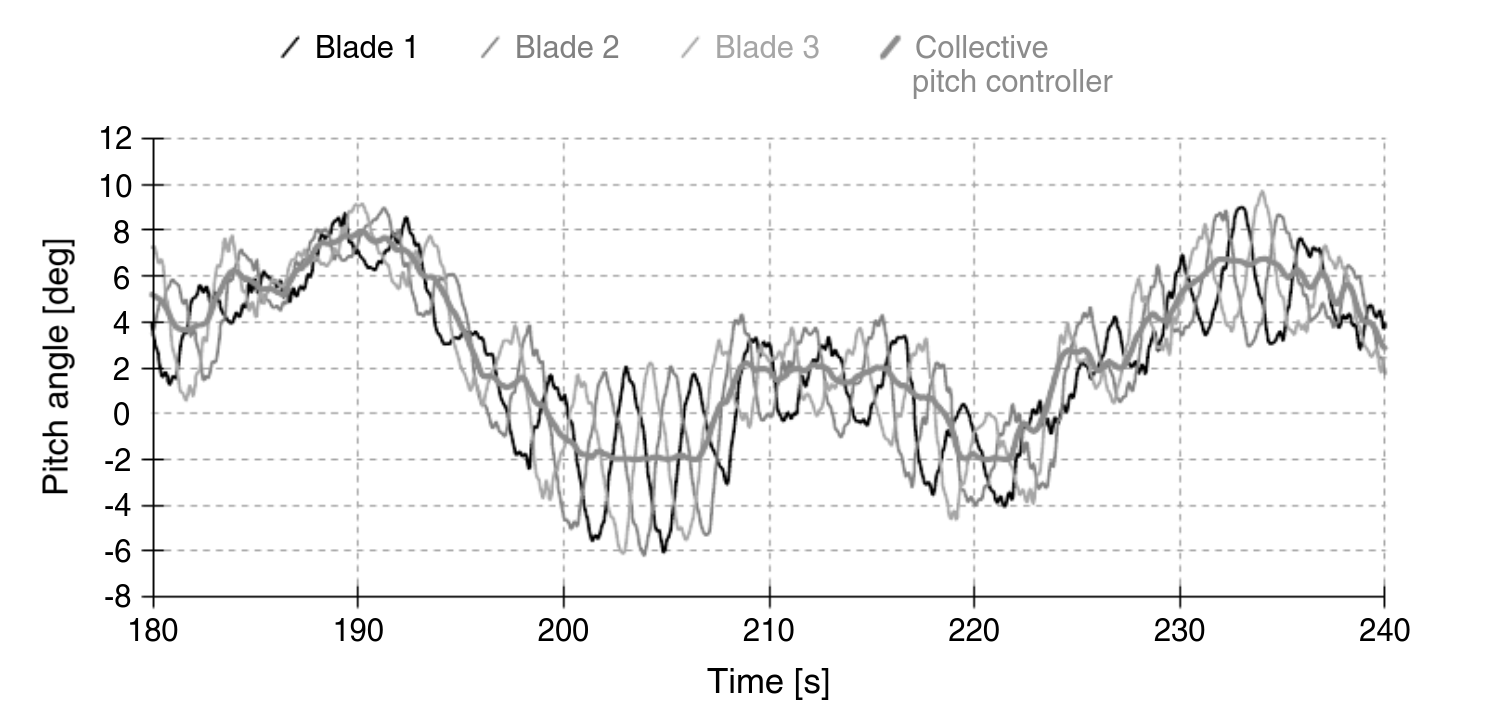
\includegraphics[width=\textwidth]{images/IPC-reference.png}
  \caption{An example pitch plot taken from \citet[Figure 2]{bossanyiIndividualBladePitch2003} for an IPC controller for a 5MW turbine in a turbulent wind scenario.}
  \label{fig:ipc-reference}
\end{figure}

As visible in Figure \ref{fig:ipc-reference}, this strategy results in a three-phase sinusoidal actuation of the three blades, with the center of the sine being the collective pitch action. In the plot, both the collective pitch action and the IPC amplitude change over time due to changes in the incoming wind. A higher pitch angle corresponds to a higher incoming wind speed. If a high difference between top and bottom loads is encountered, the resulting sine has a high amplitude, while low load differences create a low amplitude sine. In the steady wind, most of the load differences are caused by wind shear. Hence, positive deviations from collective pitch happen mostly in the upper half of the rotation, while the negative deviation happens in the lower half of the rotation. In the turbulent wind, large turbulence eddies or spontaneous inflow angle changes can have both tilting and yawing effects resulting in a more chaotic pitching pattern. The center of the sines, the baseline collective pitch actuation, is determined as usual, e.g. through a \ac{PID} controller to regulate rotor speed.

The d-q Axis Transformation is closely related to the \textit{Coleman Transformation} \cite{birMultibladeCoordinateTransformation2008}. The Coleman Transformation can be thought of as an extension to the $c_d$-$c_q$ Axis Transformation by an additional parameter $c_s$ which marks a constant offset independent of the azimuth angle. The forward transform of a first order Coleman Transformation works as described in Equation \ref{eq:coleman-forward} and the backward transform as in \ref{eq:coleman-backward}. 

\begin{equation}
  \begin{pmatrix}
    c_s \\ c_d \\ c_q
  \end{pmatrix}
  =
  \begin{pmatrix}
    \frac{1}{3} & \frac{1}{3} & \frac{1}{3} \\
    \frac{2}{3} \cos(\sazi) & \frac{2}{3} \cos(\sazi + \frac{2\cpi}{3}) & \frac{2}{3} \cos(\sazi + \frac{4\cpi}{3}) \\
    \frac{2}{3} \sin(\sazi) & \frac{2}{3} \sin(\sazi + \frac{2\cpi}{3}) & \frac{2}{3} \sin(\sazi + \frac{4\cpi}{3})
  \end{pmatrix}
  \begin{pmatrix}
    \soopbenda \\
    \soopbendb \\
    \soopbendc
  \end{pmatrix}
  \label{eq:coleman-forward}
\end{equation}

\begin{equation}
  \begin{pmatrix}
    \apitchad \\
    \apitchbd \\
    \apitchcd
  \end{pmatrix}
  =
  \begin{pmatrix}
    1 & \cos(\sazi + \philead) & \sin(\sazi + \philead) \\
    1 & \cos(\sazi + \philead + \frac{2\cpi}{3}) & \sin(\sazi + \philead + \frac{2\cpi}{3}) \\
    1 & \cos(\sazi + \philead + \frac{4\cpi}{3}) & \sin(\sazi + \philead + \frac{4\cpi}{3})
  \end{pmatrix}
  \begin{pmatrix}
    c_S \\ c_D \\ c_Q
  \end{pmatrix}
\label{eq:coleman-backward}
\end{equation}

The backward transformation offers an azimuth offset angle $\philead$, which can be used to modify the coordinate system of the backtransform slightly. Slow acting pitch actuators can this way receive their signal a little before they reach the point of the rotation where the signal should be applied. The extended Coleman transformation offers extra freedom over the $c_d$-$c_q$ transformation, which can yield better control strategies. For an example design process, see \citet{luAnalysisDesignColeman2015}.

\subsection{Damage Equivalent Loads}
\label{section:damage-equivalent-loads}

\begin{summary}
This subsection presents an evaluation metric widely used in wind turbine research, the \acf{DEL}. Lower \acsp{DEL} are closely related to reduced long-term component wear, which is an important aim of load minimization. DELs can be computed for different components, taking into account their respective material properties.
\end{summary}

As a meaningful metric for load comparison, \acfp{DEL} has become a defacto standard in wind turbine control. \acp{DEL} are calculated using the \textit{rainflow counting} algorithm \cite{matsuichiFatigueMetalsSubjected1968} combined with the Palgrem-Miner rule \cite{minerCumulativeDamageFatigue1945}. The algorithm takes as input a time series and outputs a bending moment value that creates the same damage when applied for the same duration to the same material at a given frequency as the time series. More intuitively, when a component like a blade experiences some really high loads and a lot of smaller loads across a time series, the resulting DEL would lay somewhere in between, as a repeated loading in between would induce the same amount of damage to the blade. There are a series of assumptions for DELs to be accurate and some corrections to make up for violated assumptions, such as the Goodman correction \cite[Equation 29]{haymanMLifeTheoryManual2012}. In this work, the uncorrected \ac{DEL} calculation is used, as they form a standard in academia and industry to quickly and easily compare control strategies.

To compute the metric, load cycles over a signal are extracted through \textit{Rainflow-Counting} \cite{matsuichiFatigueMetalsSubjected1968}. A load cycle in this sense is the bending of a component one way (half cycle) or back and forth (full cycle). Rainflow-Counting returns, among other metrics, load cycle ranges $\rainflowrange$ and counts $\rainflowcount$ for all load cycles $i$ in the signal $x$. Furthermore, most Rainflow implementations offer a binning, where ranges close to each other are binned to the same range with a higher count. The Formula for calculating the damage equivalent load given the rainflow counting results after \citet[Equation 26, 30]{haymanMLifeTheoryManual2012} is described in Equation \ref{eq:del}:

\begin{equation}
  \del(x, \woehler, \fdel) = \left( \frac{\sum_i{(\rainflowcount (\rainflowrange)^\woehler})}{\fdel T_x} \right)^{\frac{1}{\woehler}}
  \label{eq:del}
\end{equation}

with $\woehler$ being the Wöhler exponent, which is specific to the component materials subjected to the loads, $T_x$ being the total simulation time of the signal in seconds, and $\fdel $ being the DEL frequency. This frequency is the aforementioned frequency, to which all loads in the signal shall be mapped. The Wöhler exponent is a single number, which approximates a \textit{SN-curve}. This curve characterizes the number of load cycles (\textit{N}) for a stress force (\textit{S}) required for the component to break. Knowledge of an SN-curve for a material type or component makes it possible to predict the time to failure under known fatigue loads. Through the Wöhler exponent, the SN-curve of a component is modeled into the DEL calculation, where a higher exponent means a lower sensitivity to low-magnitude stresses and a higher sensitivity to extreme-load stresses. \cite{blasquesMeanLoadEffects2013} \cite{freeburyDeterminingEquivalentDamage2000}

